% This file was converted to LaTeX by Writer2LaTeX ver. 1.0.2
% see http://writer2latex.sourceforge.net for more info
\documentclass[twoside,letterpaper]{article}
\usepackage{amsmath}
\usepackage{amssymb,amsfonts,textcomp}
\usepackage{array}
\usepackage[english]{babel}
\usepackage[small,bf]{caption}
\usepackage{color}
\usepackage[T1]{fontenc}
\usepackage{hhline}
\usepackage{hyperref}
\usepackage[latin1]{inputenc}
\usepackage{lscape}
\usepackage{multirow}
\usepackage{supertabular}
\hypersetup{pdftex, colorlinks=true, linkcolor=blue, citecolor=blue, filecolor=blue, urlcolor=blue, pdftitle=SYSTEMS AND SOFTWARE REQUIREMENTS SPECIFICATION (SSRS) TEMPLATE, pdfauthor=Clinton Jeffery, pdfsubject=, pdfkeywords=}
\usepackage[pdftex]{graphicx}
% Outline numbering
\setcounter{secnumdepth}{5}
\renewcommand\thesection{\arabic{section}}
\renewcommand\thesubsection{\arabic{section}.\arabic{subsection}}
\renewcommand\thesubsubsection{\arabic{section}.\arabic{subsection}.\arabic{subsubsection}}
\renewcommand\theparagraph{\arabic{section}.\arabic{subsection}.\arabic{subsubsection}.\arabic{paragraph}}
\renewcommand\thesubparagraph{\arabic{section}.\arabic{subsection}.\arabic{subsubsection}.\arabic{paragraph}.\arabic{subparagraph}}
\makeatletter
\newcommand\arraybslash{\let\\\@arraycr}
\makeatother
% Page layout (geometry)
\setlength\voffset{-1in}
\setlength\hoffset{-1in}
\setlength\topmargin{0.5in}
\setlength\oddsidemargin{1in}
\setlength\evensidemargin{1in}
\setlength\textheight{8.278in}
\setlength\textwidth{6.5in}
\setlength\footskip{0.561in}
\setlength\headheight{0.5in}
\setlength\headsep{0.461in}
% Footnote rule
\setlength{\skip\footins}{0.0469in}
\renewcommand\footnoterule{\vspace*{-0.0071in}\setlength\leftskip{0pt}\setlength\rightskip{0pt plus 1fil}\noindent\textcolor{black}{\rule{0.25\columnwidth}{0.0071in}}\vspace*{0.0398in}}
% Pages styles
\makeatletter
\newcommand\ps@Standard{
  \renewcommand\@oddhead{ University of Idaho CS Department Instructional Use\hfill \hfill NOT FOR RELEASE}
  \renewcommand\@evenhead{\@oddhead}
  \renewcommand\@oddfoot{{\textcolor{black}{SSRS Page }}{\textcolor{black}{\thepage{}}}}
  \renewcommand\@evenfoot{\@oddfoot}
  \renewcommand\thepage{\arabic{page}}
}

%% ENVIRONMENT TO SINGLE-SPACE ENUMERATION LINES
\newenvironment{my_enumerate}{
\begin{enumerate}
  \setlength{\itemsep}{1pt}
  \setlength{\parskip}{0pt}
  \setlength{\parsep}{0pt}}{\end{enumerate}
}
%% ENVIRONMENT TO SINGLE-SPACE ITEMIZED LINES
\newenvironment{my_itemize}{
\begin{itemize}
  \setlength{\itemsep}{1pt}
  \setlength{\parskip}{0pt}
  \setlength{\parsep}{0pt}}{\end{itemize}
}

\newcommand\ps@Convertviii{
  \renewcommand\@oddhead{}
  \renewcommand\@evenhead{\@oddhead}
  \renewcommand\@oddfoot{}
  \renewcommand\@evenfoot{\@oddfoot}
  \renewcommand\thepage{\arabic{page}}
}
\newcommand\ps@Convertvii{
  \renewcommand\@oddhead{}
  \renewcommand\@evenhead{\@oddhead}
  \renewcommand\@oddfoot{}
  \renewcommand\@evenfoot{\@oddfoot}
  \renewcommand\thepage{\arabic{page}}
}
\newcommand\ps@Convertvi{
  \renewcommand\@oddhead{}
  \renewcommand\@evenhead{\@oddhead}
  \renewcommand\@oddfoot{}
  \renewcommand\@evenfoot{\@oddfoot}
  \renewcommand\thepage{\arabic{page}}
}
\newcommand\ps@Convertv{
  \renewcommand\@oddhead{}
  \renewcommand\@evenhead{\@oddhead}
  \renewcommand\@oddfoot{}
  \renewcommand\@evenfoot{\@oddfoot}
  \renewcommand\thepage{\arabic{page}}
}
\newcommand\ps@Convertiv{
  \renewcommand\@oddhead{}
  \renewcommand\@evenhead{\@oddhead}
  \renewcommand\@oddfoot{}
  \renewcommand\@evenfoot{\@oddfoot}
  \renewcommand\thepage{\arabic{page}}
}
\newcommand\ps@Convertii{
  \renewcommand\@oddhead{}
  \renewcommand\@evenhead{\@oddhead}
  \renewcommand\@oddfoot{}
  \renewcommand\@evenfoot{\@oddfoot}
  \renewcommand\thepage{\arabic{page}}
}
\newcommand\ps@FirstPage{
  \renewcommand\@oddhead{}
  \renewcommand\@evenhead{\@oddhead}
  \renewcommand\@oddfoot{}
  \renewcommand\@evenfoot{\@oddfoot}
  \renewcommand\thepage{\arabic{page}}
}
\makeatother
\pagestyle{Standard}
\setlength\tabcolsep{1mm}
\renewcommand\arraystretch{1.3}
% footnotes configuration
\makeatletter
\renewcommand\thefootnote{\arabic{footnote}}
\makeatother
\title{SYSTEMS AND SOFTWARE REQUIREMENTS SPECIFICATION (SSRS) TEMPLATE}
\author{Clinton Jeffery}
\date{2010-11-18T11:33:37.30}
\begin{document}




\clearpage
{\centering\bfseries
SYSTEMS AND SOFTWARE \ REQUIREMENTS SPECIFICATION (SSRS) FOR
\par}


\bigskip

{\centering\bfseries Phunctional UML Editor \\(pUML)
\par}


\bigskip


\bigskip


\bigskip

\begin{figure}
\centering

\includegraphics[width=3.5in]{uidahologo.jpg}
\end{figure}

\bigskip


\bigskip

{\centering\bfseries Version 0.11 
\par}

{\centering\bfseries May 7, 2012 
\par}


\bigskip


\bigskip

{\centering\bfseries Prepared for: 
\par}

{\centering\bfseries Dr. Clint Jeffery
\par}

\bigskip


\bigskip

{\centering\bfseries Prepared by:
\par}

{\centering\bfseries
Josh Armstrong
\\Zach Curtis
\\Brian Bowles
\\Logan Evans
\\Jeremy Klas
\\Nathan Krussel
\\Maxine Major
\\Morgan Weir
\\David Wells
\par}

{\centering\bfseries University of Idaho \par}

{\centering\bfseries Moscow, ID \ 83844-1010 \par}




\clearpage{\centering\bfseries pUML SSRS \par}


\bigskip


{\centering\bfseries RECORD OF CHANGES \par}


\bigskip

\begin{flushleft}
\tablehead{}
\begin{supertabular}[c]{|m{0.75in}|m{1.0in}|m{1.5in}|m{0.25in}|m{2in}|c|}
\hline

\centering \bfseries Change
\centering \bfseries Number
&

\centering \bfseries Date
\par
&

\centering \bfseries Location of change\newline
\centering \bfseries(e.g., page or figure \#)
&

\centering \bfseries A\newline
\centering \bfseries M\newline
\centering \bfseries D  
&

\centering \bfseries Brief description\newline
\centering \bfseries of change
&
\bfseries Initials
\\\hline

\centering 1
& 12/10/2011
& Section 3
& \centering A
& Text material for section 3 of the SSRS document.
& LE

\\\hline
\centering 2
& 01/17/2012
& ~
& \centering A
& Added updated SSRS/SSDD pdf and TeX files
& MM

\\\hline
\centering 3
& 02/01/2012
& SSRS Document
& \centering M
& Updated SSRS
& MM

\\\hline
\centering 4
& 02/15/2012
& Section 3
& \centering M
& Use cases expanded and descriptions added
& MM

\\\hline
\centering 5
& 02/23/2012
& Section 3
& \centering M
& Use case descriptions completed
& MM

\\\hline
\centering 6
& 04/04/2012
& Section 3
& \centering M
& Revised use case descriptions
& MW

\\\hline
\centering 7
& 04/09/2012
& Section 2
& \centering A
& Requirements update
& MM

\\\hline
\centering 8
& 04/23/2012
& Section 2.1
& \centering A
& Incorporated Test Plan breakdown of requirements
& MM

\\\hline
\centering 9
& 04/30/2012
& Section 2.1 
& \centering M
& Update reqs traceability section 
& MM

\\\hline
\centering 10
& 04/30/2012
& Section 4 
& \centering M
& Merge restore and open feature descriptions   
& MM

\\\hline
\centering 11
& 04/30/2012
& Section 3.2.1
& \centering M
& Update all use cases and descriptions
& MM

\\\hline
\centering 12
& 05/07/2012
& 
& \centering M
& Modify use cases
& MM

\\\hline
\end{supertabular}
\end{flushleft}


{ {*}{\textbf{A}}{ - ADDED \ }{\textbf{M}}{ - MODIFIED \ }{\textbf{D}}{ - DELETED}}






\clearpage

{\centering\bfseries TABLE OF CONTENTS \par}


\tableofcontents


\bigskip

\bigskip

\setcounter{page}{1}\pagestyle{Convertiv}





\clearpage\clearpage\setcounter{page}{1}\pagestyle{Convertii}
\section[Introduction]{\bfseries
Introduction}

\subsection[IDENTIFICATION]{\bfseries
IDENTIFICATION}
{
The software system being considered for development is referred to as Phunctional UML Editor (pUML). \ The customer providing specifications
for the system is Dr. Clint Jeffery at the University of Idaho. \ The ultimate
customer, or end-user, of the system will be University of Idaho Computer Science students and/or faculty. \ This is a new project effort, so the version under development is version 0.9.
\newline Version 1.0 will be completed upon pUML release date.}

\subsection[PURPOSE]{\bfseries
PURPOSE}
{
The purpose of the system under development is to create and store UML diagrams.
\newline The pUML software will be used by Computer Science students at the University of Idaho, and is intended to be read and understood by the same.}

\subsection[SCOPE]{\bfseries
SCOPE}
{
The pUML software was conceptualized as a Software Engineering class project, and following its launch in September 2011, spanned nine months and a total of ten software engineering students. The pUML project will be considered finalized as of May 7, 2012, and will not have aquirers or support agencies as of the date of release. 

\bigskip

Upon completion, the pUML software will be available only for distribution to the University of Idaho Computer Science department.  The pUML software will no longer be supported by the initial software development team, and will be supported only at the direction of University of Idaho Computer Science faculty. }

\subsection[DEFINITIONS, ACRONYMS, AND
ABBREVIATIONS]{\bfseries
DEFINITIONS, ACRONYMS, AND ABBREVIATIONS}

\bigskip

\begin{flushleft}
\tablehead{}
\begin{supertabular}{|m{1.3587599in}|m{5.00806in}|}
\hline
\centering \bfseries Term or
Acronym &
\centering\arraybslash \bfseries
Definition\\\hline
 Alpha test &
 Limited release(s) to selected,
outside testers\\\hline
 Beta test &
 Limited release(s) to cooperating
customers wanting early access to developing systems\\\hline
 Final test &
 aka, Acceptance test, release of
full functionality to customer for approval
\\\hline
 SSDD &
 System and Software Design Document\\\hline
 SSRS &
 System and Software Requirements
Specification\\\hline

\end{supertabular}
\end{flushleft}
\subsection[REFERENCES]{\bfseries
REFERENCES}
{
The pUML requirements will be addressed in the following documents: 

\begin{itemize}
\item Test Plan (TP), Version 2.0
\item System and Software Design Description (SSDD) Version 0.0
\end{itemize}

}

\subsection[OVERVIEW AND RESTRICTIONS]{\bfseries
OVERVIEW AND RESTRICTIONS}
{
This document is for limited release only to University of Idaho Computer Science personnel assigned to the pUML project.
}


\bigskip

{
Section 2 of this document describes the system under development from a holistic point of view. 
\newline Functions, characteristics, constraints, assumptions, dependencies, and overall requirements are defined from the system-level perspective.
}


\bigskip

{
Section 3 of this document describes the specific requirements of the
system being developed. \ Interfaces, features, and specific
requirements are enumerated and described to a degree sufficient for a
knowledgeable designer or coder to begin crafting an architectural
solution to the proposed system.}


\bigskip

{
Section 4 provides the requirements traceability information for the
project. \ Each feature of the system is indexed by the SSRS
requirement number and linked to its SDD and test references.}




\clearpage\section[OVERALL DESCRIPTION]{\bfseries
OVERALL DESCRIPTION}

\subsection[PRODUCT PERSPECTIVE]{\bfseries
PRODUCT PERSPECTIVE}
{
This product is independent of any other product, and as such, is self-contained.
}

\subsection[PRODUCT FUNCTIONS ]
{\bfseries PRODUCT FUNCTIONS}

This product's primary function is to allow the user to create UML diagrams, edit existing diagrams, and store and retrieve them. \newline 
Features to be tested include all objects, connectors, and associated functionality, Open/Save functionality, and all diagram types load properly. The specific requirements for the UML diagram editor are itemized insubsequent sections. 

\bigskip


\subsubsection[INSTALL / LAUNCH / EXIT]
{\bfseries INSTALL / LAUNCH / EXIT}

Basic functionality that must be met prior to use of this software involves the successful installation and launch of the pUML software:
\begin{itemize}
\item pUML software includes an installer, which at basic functionality will:
\begin{itemize}
\item Consist of a single downloadable installation file.
\item Install on Windows and Linux platforms, resulting in a single application icon.
\item Uninstall from both Windows and Linux platforms.
\end{itemize}
\item Once installed, the pUML software may be launched by double-clicking the pUML icon.
\item pUML may be exited by clicking an "X" in the upper corner of the software, or by selecting "File,"  and then "Exit." 
\end{itemize}

\bigskip


\subsubsection[MENU OPTIONS / MAIN WINDOW]
{\bfseries MENU OPTIONS / MAIN WINDOW} 
{
\begin{itemize}
\item Options window appears at pUML startup.
\item When the options window is closed with no selections made, the pUML main window remains.
\item When "New" is selected, options window appears.
\item When "Open" is selected, an explorer window appears.
\item When "Save" is selected: refer to subsection 2.1.6.
\item When "Save As.." is selected: refer to subsection 2.1.6.
\item When Exit is clicked:
\begin{itemize}
\item If all currently open diagrams are saved, pUML exits.
\item If any open diagram is not saved, refer to subsection 2.1.6.
\end{itemize}
\end{itemize}
\bigskip

\subsubsection[OBJECTS]{\bfseries OBJECTS} 

All objects should perform or have the following tasks performed on them in a consistent manner in the following cases: 
\begin{itemize}
	\item Objects can be created.
	\item Objects can be deleted.
\begin{itemize}
\item Any associated connectors must also be deleted.
\item All associated text and descriptions must also be deleted.
\end{itemize}
	\item Objects can be selected.
	\item Objects can be de-selected.
	\item Objects can be moved after they have been placed
\begin{itemize}
\item Objects moved retain the new location after the associated diagram is saved, closed, and restored.
\item All text and descriptions associated with the object move with the object to the same location in relation to the object.
\end{itemize}
\item Objects can accept an indefinite number of connection lines.
\item The object`s properties may be modified an indefinite number of times.
\item The object will automatically resize to fit the contents.
\end{itemize}

\bigskip

\subsubsection[CONNECTORS]{\bfseries CONNECTORS}

All connectors should perform or have the following tasks performed on them in a consistent manner in the following cases: 
\begin{itemize}
\item Connectors can be created.
\begin{itemize}
\item Only one connector may exist between any two objects.
\item Only one self connector may exist per object.
\end{itemize}
\item Connectors can be deleted.
\item Connectors can be selected.
\item Connectors can be de-selected.
\item Connectors cannnot be moved from one object and placed onto another. 
\item If an object a connector is attached to moves, the connector's endpoint attached to that object will move with that object. 
\begin{itemize}
\item Connectors moved retain the new configuration with the same integrity as the previous configuration.
\item All text and descriptions associated with the connector move with the connector to the same location in relation to the connector as before.
\end{itemize}
\item The connector's properties may be modified.
\begin{itemize}
\item Line description may be modified an indefinite number of times.
\end{itemize}
\end{itemize}

\bigskip

\subsubsection[OPEN]{\bfseries OPEN}

Once the pUML software has been launched, files may be opened if the following criteria are met:

\begin{itemize}
\item The file type is of pUML type.
\item The file name is legitimate.
\item The file is not already open in pUML.
\end{itemize}

\bigskip

Note: The cases listed above are ensured by QT, and will not be tested.
\newline 


If the user opens a pUML diagram file, restore functionality will occur as follows:
\begin{itemize}
\item If the pUML software is not already loaded, it will load.
\item A new tab will open, and the previously saved diagram will appear in the tab.
\item The toolbar is updated with that diagram's objects and connectors.
\item All objects and connectors in the file are in the exact same state and configuration as when the file had been previously saved.
\item The file may be modified (edited).
\begin{itemize}
\item Objects may be added or removed.
\item Connectors may be added or removed.
\end{itemize}
\item The file may be saved.
\item The file may be closed.
\end{itemize}

\bigskip

\subsubsection[SAVE]{\bfseries SAVE/SAVE AS}
{
The Save and Save As functions may be invoked if the following criteria are met: 
\begin{itemize}
\item A diagram is open in pUML.
\end{itemize}
}

\bigskip

Save/Save As functionality:
\newline
{
\begin{itemize}
\item A diagram may be saved regardless of whether it is new or previously saved.
\item A diagram may be saved whether or not it has been modified. (e.g., a blank diagram may be saved)
\item If a diagram has been previously saved, pUML will automatically write over the saved file's contents. The modified diagram will be saved at the original location of the diagram under the original name.
\item If a diagram has not been previously saved, Save As will automatically occur.
\begin{itemize}
\item The Save-As dialog will load.
\item The user must select an appropriate file name and storage location. 
\item The diagram will be stored at the location and under the name the user has entered.
\end{itemize}
\end{itemize}
}

\bigskip


\subsubsection[DIAGRAM TYPES]{\bfseries DIAGRAM TYPES}

\begin{itemize}
\item pUML diagrams may be of only one diagram type. (There are no legitimate UML diagrams that combine elements of more than one diagram type)
\item Diagram-specific objects and connectors will be the only ones displayed in the toolbar for a specific diagram type.
\item The type of the diagram will be saved with a diagram file, so that a diagram may not be loaded into a tab with a different diagram type.
\end{itemize}


\bigskip

\subsubsection[TAB FUNCTIONALITY]{\bfseries TAB FUNCTIONALITY}

\begin{itemize}
\item Except for the initial loading of pUML (initial options window view), at least one tab must be open at any time.
\item If all tabs are closed, pUML exits.
\item If the diagram loaded into a tab is saved, clicking the ``X'' will close the tab.
\item If the diagram loaded into a tab is not saved, and the ``X'' is clicked: refer to subsection 2.1.6.
\item pUML will permit an indefinite number of tabs to be opened at any time, but this may consume a disproportionate amount of resources.
\end{itemize}



\bigskip




}

\subsection[USER CHARACTERISTICS]{\bfseries
USER CHARACTERISTICS}
{
The intended user for the pUML software are software engineers and computer science students with a prior knowledge of UML. This user is already familiar with computers and generally has some experience in programming languages.
}

\subsection[CONSTRAINTS]{\bfseries
CONSTRAINTS}
{
Since the pUML project was developed as a class assignment,
further development of this project will halt if the University of Idaho faculty overseeing this project decide that this project should to no longer continue.
}

\subsection[ASSUMPTIONS AND DEPENDENCIES]{\bfseries
ASSUMPTIONS AND DEPENDENCIES}
{
The requirements for the pUML software were decided upon by University of Idaho Computer Science Department faculty.  Any further direction this project may take will depend on their decisions. As of this revision, it is currently undecided if this project will be maintained after the corresponding course has concluded. 
}




\subsection[SYSTEM LEVEL (NON{}-FUNCTIONAL)
REQUIREMENTS]{\bfseries
SYSTEM LEVEL (NON-FUNCTIONAL) REQUIREMENTS}

\subsubsection[Site dependencies]{\bfseries
Site dependencies}
{
The pUML software has no dependencies on any external resources, such as internet access, etc..
Any modern operating system (2008+) should be sufficient to support the pUML software,
and since this software is cross-platform, there should be no complications.
}

\subsubsection[Safety, security and privacy requirements]{\bfseries
Safety, security and privacy requirements}
{
There are no safety, security or privacy requirements at this time.
}

\subsubsection[Performance requirements]{\bfseries
Performance requirements}
{
This software is to be supported on one terminal per install, and since there are no current
 limitations applying to product distribution, it may be installed on a theoretically infinite 
number of terminals. This software is not designed to be remotely accessed, and as a result, 
one user per session is recommended as well.  The software has not been tested to determine 
efficient transaction times as of the date of this SSRS publication.
}

\subsubsection[System and software quality]{\bfseries System
and software quality}
{
The fully developed software should be available for use and reliably handle all requests 98 
percent of the time.  The software can currently handle saving, diagram selection, allow for 
editing of multiple diagrams at a time, diagram component deletion, diagram component labeling, 
and loading of saved diagrams.
}

\subsubsection[Packaging and delivery requirements]{\bfseries
Packaging and delivery requirements}
{
The executable system and all associated documentation (i.e., SSRS, SSDD, code listing, test plan (data and results), and user manual) will be delivered to the customer on CD{\textquoteright}s and/or via email, as
specified by the customer at time of delivery. \ Although the user will be kept informed of progress via the Mercurial repository throughout the
system development process, the final, edited version of the above
documents will accompany the final, accepted version of the executable
system.}

\subsubsection[Personnel{}-related requirements]{\bfseries
Personnel-related requirements}
{
The system under development has no special personnel-related
characteristics. }

\subsubsection[Training{}-related requirements]{\bfseries
Training-related requirements}
{
A user manual will be included in this project to aid users who have difficulty intuiting the proper action to produce the corresponding outcome.
}

\subsubsection[Logistics{}-related requirements]{\bfseries
Logistics-related requirements}
{
The pUML software is intended for use on University of Idaho Computer Science department computers as well as computer science students' personal computers including, at a minimum, operating systems Windows 7, Mac OSX, and Linux.
Any minimum hardware requirements lie outside the scope of the resources available,
and there will be no software application dependencies at the time of release.
}

\subsubsection[Precedence and criticality of requirements]{\bfseries
Precedence and criticality of requirements}
{
System and software quality are the primary focus of our software development. All additional features and functionality are secondary. 
}












\clearpage\section[SPECIFIC REQUIREMENTS]{\bfseries
SPECIFIC REQUIREMENTS}

\subsection[EXTERNAL INTERFACE REQUIREMENTS]{\bfseries
EXTERNAL INTERFACE REQUIREMENTS}

\subsubsection[Hardware Interfaces]{\bfseries
Hardware Interfaces}
{

{
Any computing system capable of running Linux or Windows 7.}}

\subsubsection[Software Interfaces]{\bfseries
Software Interfaces}
{ 
{
Either a Linux or Windows 7 operating system to guarantee functionality.
}}

\subsubsection[User Interfaces]{\bfseries
User Interfaces}
{
The only user interfaces required to operate the pUML software are standard computing interfaces
\begin{itemize}
  \item Monitor
  \item Keyboard
  \item Mouse
\end{itemize}
}

\subsubsection[Other Communication
Interfaces]{\bfseries
Other Communication Interfaces}
{
{No other interfaces are required. }}





\clearpage\setcounter{page}{1}\pagestyle{Convertv}

\subsection[SYSTEM FEATURES]{\bfseries
SYSTEM FEATURES}


\subsubsection{Use Cases and Descriptions}
{The following use cases represent different stages at which options will be available to the user.}

\bigskip

% ************************************
% LAUNCH USE CASE & DESCRIPTIONS
% ************************************
\paragraph[\ Use Category]
{\ Launch} {These options will be available to the user upon the launch of pUML.}

\begin{figure}[h]
\centering
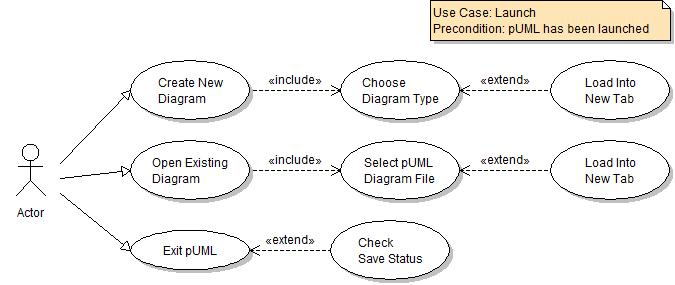
\includegraphics[width=6.0in]{ucaseLaunch.jpg}
\caption{Launch Use Case}
\end{figure}

%%% CREATE NEW DIAGRAM USE CASE DESCRIPTION
\begin{flushleft}
\tablehead{}
\begin{tabular}{|m{2.0in} m{5.0in}|}
\hline
{\bfseries\emph{Use Case Name}}
& {\bfseries Create New Diagram }
\\\hline
\emph{Participating Actor}
& User
\\\hline
\emph{Flow of Events}
& \begin{my_enumerate}
\item The user selects ``New'' from menu.
\item Program requests user select a diagram type.
\item The program responds by creating a new tab with a blank drawing canvas.
\item Program loads and displays only objects for the selected diagram type.
\end{my_enumerate}
\\\hline
\emph{Entry Condition}
& User selects ``New'' from commands
\\\hline
\emph{Exit Condition}
& Program successfully opens new tab with diagram specific tools in toolbar.
\\\hline
\emph{Quality Requirements}
& Toolbar loads only diagram specific objects and connectors.
\\\hline
\end{tabular}
\end{flushleft}

\bigskip

%%% OPEN EXISTING DIAGRAM USE CASE DESCRIPTION
\begin{flushleft}
\tablehead{}
\begin{tabular}{|m{2.0in} m{5.0in}|}
\hline
{\bfseries\emph{Use Case Name}}
& {\bfseries Open Existing Diagram}
\\\hline
\emph{Participating Actor}
& User
\\\hline
\emph{Flow of Events}
& \begin{my_enumerate}
\item User selects ``Open'' from menu.
\item Program opens an explorer window.
\item User selects the file they wish to open.
\item Program loads selected file into a new tab.
\end{my_enumerate}
\\\hline
\emph{Entry Condition}
& User selects ``Open'' from menu.
\\\hline
\emph{Exit Condition}
& File is successfully opened into a new tab.
\\\hline
\emph{Quality Requirements}
& User selected file must be of pUML diagram type.\newline
  Only diagram-appropriate tools loaded into toolbar.
\\\hline
\end{tabular}
\end{flushleft}

\bigskip


%%% EXIT PROGRAM USE CASE DESCRIPTION
\begin{flushleft}
\tablehead{}
\begin{tabular}{|m{2.0in} m{5.0in}|}
\hline
{\bfseries\emph{Use Case Name}}
& {\bfseries Exit pUML}
\\\hline
\emph{Participating Actor}
& User
\\\hline
\emph{Flow of Events}
& \begin{my_enumerate}
\item User clicks X.
\item If a file is open, program checks to see if it is saved.  If no files are open, simply exits.
\item Program Exits.
\end{my_enumerate}
\\\hline
\emph{Entry Condition}
&
User initiates File menu option ``Close Program'' or clicks X in the corner of the window.
\\\hline
\emph{Exit Condition}
& File is successfully saved and the program exits.
\\\hline
\emph{Quality Requirements}
& File must be saved prior to exiting, or changes must be discarded prior to exiting. \newline
  If the current tab closed was the only tab open in pUML, pUML exits.
\\\hline
\end{tabular}
\end{flushleft}
\bigskip

\clearpage


% *****************************************
% NEW/OPEN DIAGRAM USE CASES & DESCRIPTIONS
% *****************************************
\paragraph[\ New/Open Diagram]
{\ New/Open Diagram} {These options will be available to the user after creating a new UML diagram, or upon opening an existing UML diagram. This set of use cases covers all edits possible for pUML diagrams.}

\begin{figure}[h]
\centering
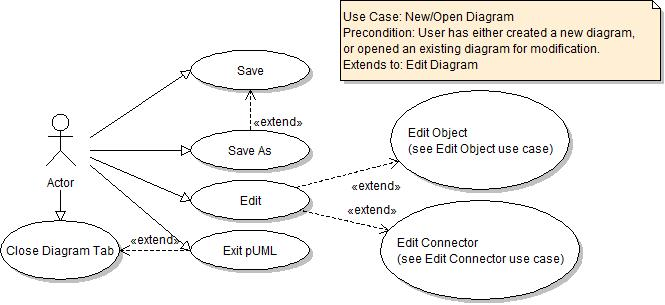
\includegraphics[width=6.0in]{ucaseNewOpenDiagram.jpg}
\caption{New/Open Diagram Use Case}
\end{figure}

%%% SAVE DIAGRAM USE CASE DESCRIPTION
\begin{flushleft}
\tablehead{}
\begin{tabular}{|m{2.0in} m{5.0in}|}
\hline
{\bfseries\emph{Use Case Name}}
& {\bfseries Save}
\\\hline
\emph{Participating Actor}
& User
\\\hline
\emph{Flow of Events}
& \begin{my_enumerate}
  \item The user opens the File menu and selects ``Save.''
  \item Program saves file under current file name 
\begin{my_enumerate}
\item If file has not been previously saved, program initiates Save As use case. 
\item If file has been previously saved, the program saves the file at its existing location under its existing name.
\end{my_enumerate}
\end{my_enumerate}
\\\hline
\emph{Entry Condition}
& User selects ``Save File'' from main menu or clicks Save button.
\\\hline
\emph{Exit Condition}
& File is successfully saved
\\\hline
\emph{Quality Requirements}
& File names must be valid \newline
  May not create two pUML diagram files with same name in same location.
\\\hline
\end{tabular}
\end{flushleft}
\bigskip


%%% SAVE DIAGRAM AS USE CASE DESCRIPTION
\begin{flushleft}
\tablehead{}
\begin{tabular}{|m{2.0in} m{5.0in}|}
\hline
{\bfseries\emph{Use Case Name}}
& {\bfseries Save As}
\\\hline
\emph{Participating Actor}
& User
\\\hline
\emph{Flow of Events}
& \begin{my_enumerate}
\item User opens File menu and selects ``Save As...''
\end{my_enumerate}
\ ~ or
\begin{my_enumerate}
\item User selects ``Save'' from File menu, but the program has not been previously saved.
\item Program displays a dialog box requesting the user to enter a diagram name and save location.
\item User enters a diagram name and clicks ``Ok.''
\item Program saves diagram at user specified location.
\end{my_enumerate}
\\\hline
\emph{Entry Condition}
& User clicks ``Save As'' or clicks ``Save'' with a previously unsaved diagram. 
\\\hline
\emph{Exit Condition}
& The diagram has been saved.
\\\hline
\emph{Quality Requirements}
& Inherited from Save use case. 
\\\hline
\end{tabular}
\end{flushleft}
\bigskip


%%% CLOSE DIAGRAM TAB USE CASE DESCRIPTION
\begin{flushleft}
\tablehead{}
\begin{tabular}{|m{2.0in} m{5.0in}|}
\hline
{\bfseries\emph{Use Case Name}}
& {\bfseries Close Diagram Tab}
\\\hline
\emph{Participating Actor}
& User
\\\hline
\emph{Flow of Events}
& \begin{my_enumerate}
\item User clicks the `X' on the diagram tab.
\item If the current version of the diagram is saved, the program closes the diagram tab.
\end{my_enumerate}
\ ~or
\begin{my_enumerate}
\item User clicks the `X' on the diagram tab.
\item If the program is not saved, the program issues a warning.
\end{my_enumerate}
\\\hline
\emph{Entry Condition}
& User clicks the ``X'' on the diagram tab.
\\\hline
\emph{Exit Condition}
& Diagram tab is closed.
\\\hline
\emph{Quality Requirements}
& Diagram must be saved for the tab to close, or the user must either choose to save the diagram or discard changes.
\\\hline
\end{tabular}
\end{flushleft}
\bigskip

\clearpage

% ************************************
% EDIT OBJECT USE CASE & DESCRIPTIONS
% ************************************
\paragraph[\ Edit Object]
{\ Edit Object} {These options will be available to the user with a diagram open for modification, who is choosing to take action on an object.}

\begin{figure}[h]
\centering
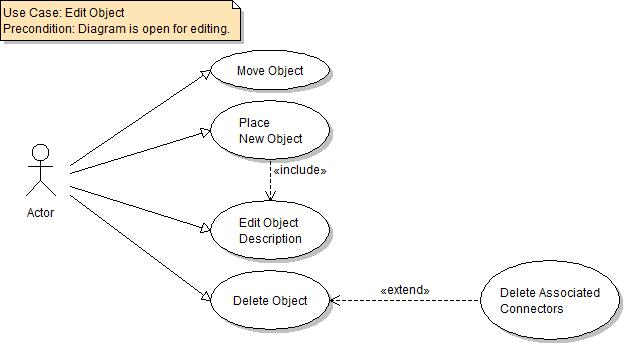
\includegraphics[width=6.0in]{ucaseEditObj.jpg}
\caption{Edit an Object Use Case}
\end{figure}

%%% PLACE NEW OBJECT USE CASE DESCRIPTION
\begin{flushleft}
\tablehead{}
\begin{tabular}{|m{2.0in} m{5.0in}|}
\hline
{\bfseries\emph{Use Case Name}}
& {\bfseries Place New Object}
\\\hline
\emph{Participating Actor}
& User
\\\hline
\emph{Flow of Events}
& \begin{my_enumerate}
\item User selects an object from toolbar.
\item User clicks the canvas.
\item Program places an object at that location on the canvas.
\item User may be prompted to enter a description for the object.
\end{my_enumerate}
\\\hline
\emph{Entry Condition}
& pUML diagram is open for editing. \newline 
Toolbar is loaded with valid objects for diagram type.
\\\hline
\emph{Exit Condition}
& Object has been successfully placed on drawing canvas.
\\\hline
\emph{Quality Requirements}
& Object must be of diagram type.
\\\hline
\end{tabular}
\end{flushleft}
\bigskip

%%% EDIT OBJECT DESCRIPTION USE CASE DESCRIPTION
\begin{flushleft}
\tablehead{}
\begin{tabular}{|m{2.0in} m{5.0in}|}
\hline
{\bfseries\emph{Use Case Name}}
& {\bfseries Edit Object Description}
\\\hline
\emph{Participating Actor}
& User
\\\hline
\emph{Flow of Events}
& \begin{my_enumerate}
\item User selects an object by clicking on it.
\item User right-clicks on the object.
\item User selects ``Properties'' from the drop-down menu.
\item User types the desired description in the text box presented.
\item User clicks ``OK.''
\item Program displays new description.
\end{my_enumerate}
\\\hline
\emph{Entry Condition}
& User right-clicks on an object and selects ``Properties'' from the dropdown menu.
\\\hline
\emph{Exit Condition}
& Object now displays new description.
\\\hline
\emph{Quality Requirements}
& N/A
\\\hline
\end{tabular}
\end{flushleft}
\bigskip


%%% MOVE OBJECT USE CASE DESCRIPTION
\begin{flushleft}
\tablehead{}
\begin{tabular}{|m{2.0in} m{5.0in}|}
\hline
{\bfseries\emph{Use Case Name}}
& {\bfseries Move Object}
\\\hline
\emph{Participating Actor}
& User
\\\hline
\emph{Flow of Events}
& \begin{my_enumerate}
\item User clicks on object, selecting it.
\item User holds down the left mouse button, and moves the mouse to the new location of the object.
\item User releases the left mouse button.
\item Program draws the object at the new location, with all attached connectors. 
\end{my_enumerate}
\\\hline
\emph{Entry Condition}
& User selects an object with the left mouse button held down.
\\\hline
\emph{Exit Condition}
& Program has drawn the object at the new location.
\\\hline
\emph{Quality Requirements}
& Connectors move with object. 
\\\hline
\end{tabular}
\end{flushleft}
\bigskip


%%% DELETE OBJECT USE CASE DESCRIPTION
\begin{flushleft}
\tablehead{}
\begin{tabular}{|m{2.0in} m{5.0in}|}
\hline
{\bfseries\emph{Use Case Name}}
& {\bfseries Delete Object}
\\\hline
\emph{Participating Actor}
& User
\\\hline
\emph{Flow of Events}
& \begin{my_enumerate}
\item User right clicks object and selects ``Delete'' from the dropdown menu.
\item Program deletes the object and all attached connectors. 
\end{my_enumerate}
\\\hline
\emph{Entry Condition}
& User right clicks object and selects ``Delete'' from the dropdown menu.
\\\hline
\emph{Exit Condition}
& Program deletes object and all attached connectors.
\\\hline
\emph{Quality Requirements}
& Attached connectors must be deleted with deleted object. 
\\\hline
\end{tabular}
\end{flushleft}
\bigskip


\clearpage

% ************************************
% EDIT CONNECTOR CASE & DESCRIPTIONS
% ************************************
\paragraph[\ Use Category]
{\ Edit Connector} {These options will be available to the user with a diagram open for modification, who is choosing to take action regarding a connector.}

\begin{figure}[h]
\centering
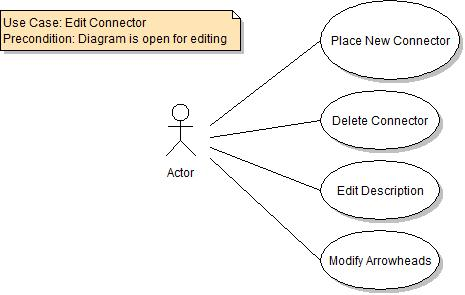
\includegraphics[width=6.0in]{ucaseEditConn.jpg}
\caption{Edit a Connector Use Case}
\end{figure}

%%% PLACE NEW CONNECTOR USE CASE DESCRIPTION
\begin{flushleft}
\tablehead{}
\begin{tabular}{|m{2.0in} m{5.0in}|}
\hline 
  {\bfseries\emph{Use Case Name}} 
  & {\bfseries Place New Connector}
\\\hline
  \emph{Participating Actor} 
  & User
\\\hline
\emph{Flow of Events}
& \begin{my_enumerate}
\item User clicks on desired connector in toolbar.
\item User clicks on the first (origination) object, holding down the left mouse button.
\item User drags the mouse to a second (destination) object.
\item User releases the mouse button.
\item Program draws the connection line between the first and second object.
\end{my_enumerate}
\\\hline
  \emph{Entry Condition}
  & User has selected a connector from the toolbar.
\\\hline
  \emph{Exit Condition}
  & The connector is successfully drawn between two objects. 
\\\hline
  \emph{Quality Requirements}
  & Only one connector may be placed between any two objects.
\\\hline
\end{tabular}
\end{flushleft}
\bigskip


%%% EDIT CONNECTOR PROPERTIES USE CASE DESCRIPTION
\begin{flushleft}
\tablehead{}
\begin{tabular}{|m{2.0in} m{5.0in}|}
\hline {\bfseries\emph{Use Case Name}}
& {\bfseries Edit Connector Properties}
\\\hline
\emph{Participating Actor}
& User
\\\hline
\emph{Flow of Events}
& 
\begin{my_enumerate}
\item User right-clicks on the connector and selects ``Properties'' from the drop-down menu.
\item User edits description in the text box presented.
\item User clicks ``OK.''
\item Program displays new line description.
\end{my_enumerate}
\\\hline
\emph{Entry Condition}
& User right-clicks on the connector and selects ``Properties'' from the drop-down menu.
\\\hline
\emph{Exit Condition}
& Program has updated the connector with the new properties.
\\\hline
\emph{Quality Requirements}
& Some connectors may not have the option to edit/modify the description.
\\\hline
\end{tabular}
\end{flushleft}
\bigskip


%%% DELETE CONNECTOR USE CASE DESCRIPTION
\begin{flushleft}
\tablehead{}
\begin{tabular}{|m{2.0in} m{5.0in}|}
\hline {\bfseries\emph{Use Case Name}}
& {\bfseries Delete Connector}
\\\hline
\emph{Participating Actor}
& User
\\\hline
\emph{Flow of Events}
& \begin{my_enumerate}
\item User right clicks on a connector and selects ``Delete'' from the drop-down menu.
\item Program deletes the connector.
\end{my_enumerate}
\\\hline
\emph{Entry Condition}
& User right clicks on a connector and selects ``Delete'' from the drop-down menu.
\\\hline
\emph{Exit Condition}
& Connector has been deleted.
\\\hline
\emph{Quality Requirements}
& Only the connector is to be deleted. Attached objects are to remain on the canvas.
\\\hline
\end{tabular}
\end{flushleft}
\bigskip



\clearpage






\subsubsection[System feature: [Project management tasks suite]{\bfseries System feature: Project management tasks suite}

\paragraph[\ Introduction/Purpose for These Features] 
{\bfseries Introduction/Purpose for These Features}
{
The features detailed in the use cases (Section 3.2.1) are all basic vital functions for a UML Diagram editor. At the most basic level, in order to create UML diagrams, several processes are required. These processes include the creation of distinct UML diagrams consisting of labeled objects and connectors, saving of these diagrams, and the ability to load these saved diagrams for modification.
}


\paragraph[Input/Output sequence for this feature]
{\bfseries Input/Output sequence for These Features}
{ All input/output sequences are detailed in associated use case descriptions in section 3.2.1.
 The purpose of each use case action is detailed below. }

\subparagraph{Create New Diagram}
{ This creates a new canvas in which the user may design a UML diagram. Since there are four different diagram types that may be created with pUML, and many design projects necessitate several diagrams, there is currently no predetermined limit on the number of new diagrams that may be created in pUML. (This is determined by system resources only, and may differ from system to system.) }

\subparagraph{Open Existing Diagram}
{ This opens a previously saved UML diagram. Since each diagram is of a specific diagram type, when a pUML diagram is loaded, only the tools available for that diagram type will be available to the user upon loading. When a diagram has been opened, the user then may modify this diagram further. There is no limit to the number of times a diagram may be modified.  There is currently no limit to the number of diagrams that may be opened into the pUML software. (This is determined by system resources only, and may differ from system to system.)  }

\subparagraph{Exit pUML}
{ The user may exit pUML by either selecting ``File'' and then ``Exit,'' or may click the ``X'' in the upper corner of the pUML main window. If any currently loaded diagrams have changes which have not been saved, pUML will request confirmation to either save or discard changes prior to exiting. }

\subparagraph{Save}
{ This saves the current state of the diagra, into an XML file that can later be used to recreate the diagram state. If the current diagram does not have a name, the ``Save'' option will be an alias for the ``Save As'' option.}

\subparagraph{Save As}
{ This prompts pUML to load a browser window. The user must select a location and a file name in which to store the pUML diagram.  After clicking ``Ok,'' the Save function completes this process.  This state will be defaulted to if the user clicks ``Save'' on a previously unsaved diagram.}

\subparagraph{Close Diagram Tab}
{ If the user clicks the ``x'' on the tab, and if the current diagram state is saved, the diagram will close. Otherwise, the ``Save As'' function will initiate prior to closing. This feature is useful to de-clutter the pUML workspace. In addition, if the closed tab was the only tab open, then the pUML software will exit.}

\subparagraph{Place New Object/Connector, Edit Object/Connector Descriptions, and Move/Delete Object/Connector}
{ UML diagrams consist of different types of objects and connectors. Each object and connector ideally have an associated description. UML diagram functionality must include the placement of objects and connectors, in addition to the ability to modify their descriptions, move their locations, and delete them as necessary. When an object is deleted, attached connectors must be deleted as well. However, if a connector is deleted, any attached objects will not be deleted. }


% **************************************
% SECTION 4: REQUIREMENTS TRACEABILITY *
% **************************************


\clearpage

\begin{landscape}

\section[REQUIREMENTS TRACEABILITY]
  {\bfseries REQUIREMENTS TRACEABILITY}
{\itshape }

\bigskip

\begin{flushleft}
\tablehead{}
\begin{supertabular}[c]{|
                        m{0.9in}|m{0.4in}|m{2.0in}|
                        m{0.4in}|m{0.5in}|m{1.0in}|
                        m{1.0in}|m{1.0in}|c|
                       }
\hline
 
  \centering \bfseries Feature Name &
  \centering \bfseries Req No. &
  \centering \bfseries Requirement Description &
  \centering \bfseries Priority &
  \centering \bfseries SSDD &
  \centering \bfseries Test Case(s) & 
  \centering \bfseries Alpha Release &
  \centering \bfseries Beta Release &
  \bfseries Final Test
\\\hline
  
  Install
  & \centering 2.2.1
  & pUML software installs successfully
  & \centering M 
  & ~
  & testinstall
  & PASS
  & ~ 
  & ~ 
\\\hline

  Launch
  & \centering 2.2.1
  & pUML software launches successfully
  & \centering M 
  & ~
  & testlaunch
  & PASS
  & ~ 
  & ~ 
\\\hline

  Exit
  & \centering 2.2.1
  & pUML Exit options 
  & \centering M 
  & ~
  & testsave *\newline
    testsaveas *
  & FAIL \newline
    FAIL 
  & ~ \newline
    ~
  & ~ \newline
    ~
\\\hline

  Main Window
  & \centering 2.2.2
  & All main window features 
  & \centering M 
  & ~
  & testmainwindow 
  & PASS
  & ~ 
  & ~ 
\\\hline

  Objects
  & \centering 2.2.3
  & Object properties and functionality
  & \centering M 
  & ~ 
  & testobjects
  & PASS
  & ~ 
  & ~ 
\\\hline

  Connectors
  & \centering 2.2.4
  & Connector properties and functionality
  & \centering M 
  & ~ 
  & testconnectors\newline 
    testselfconnector
  & FAIL \newline
    PASS
  & ~ \newline
    PASS
  & ~ \newline
    ~
\\\hline

  Open
  & \centering 2.2.5
  & Load a pUML file into pUML 
  & \centering M 
  & ~ 
  & testsave *\newline
    testsaveas *
  & FAIL \newline
    FAIL 
  & ~ \newline
    ~
  & ~ \newline
    ~
\\\hline

  Save/Save As
  & \centering 2.2.6
  & Save a diagram 
  & \centering M 
  & ~ 
  & testsave \newline 
    testsaveas
  & FAIL \newline
    PASS
  & ~ \newline
    ~
  & ~ \newline
    ~
\\\hline

  Diagrams
  & \centering 2.2.7
  & Diagram type integrity 
  & \centering M 
  & ~ 
  & testsave *\newline 
    testsaveas *
  & FAIL \newline
    FAIL
  & ~ \newline
    ~
  & ~ \newline
    ~
\\\hline

  Tabs
  & \centering 2.2.8
  & Tab functionality 
  & \centering M 
  & ~ 
  & testsave *\newline 
    testsaveas *
  & FAIL \newline
    FAIL
  & ~ \newline
    ~
  & ~ \newline
    ~
\\\hline

\end{supertabular}
\end{flushleft}

{Priorities are: \textbf{M}andatory, \textbf{L}ow, \textbf{H}igh} \newline
{SSDD link is version and page number or function name.} \newline
{Test cases and results are file names and \textbf{P}ass/\textbf  {F}ail or \% passing.} \newline
{* asterisk indicates indirectly tested through another feature test case.}

\bigskip

\end{landscape}

\end{document}
